% -*- LaTeX -*-
% -*- coding: utf-8 -*-
%
% ~~~~~~~~~~~~~~~~~~~~~~~~~~~~~~~~~~~~~~~~~~~~~~~~~~~~~~~~~~~~~~~~~~~~~~~~~~~~~~
%
%                             michael a.g. aïvázis
%                      california institute of technology
%                      (c) 1998-2010  all rights reserved
%
% ~~~~~~~~~~~~~~~~~~~~~~~~~~~~~~~~~~~~~~~~~~~~~~~~~~~~~~~~~~~~~~~~~~~~~~~~~~~~~~
%

\lecture{Structured grids}{20100208}

% --------------------------------------
% overview
\begin{frame}[fragile]
%
  \frametitle{Overview}
%
  \begin{itemize}
%
  \item lattices: logically Cartesian grids
    \begin{itemize}
    \item flow, lattice dynamics, wave propagation, image processing
    \end{itemize}
%
  \item suitable when it is possible to find an invertible map $\phi$ from the problem domain
    $\Omega$ to $\mathbb{Z}^{d}$
%
  \item data representation: multi-dimensional arrays
    \begin{itemize}
    \item $\phi$ maps points in $\Omega$ to loop indices
    \item with {\em guard cells} for enforcing boundary conditions
    \end{itemize}
% 
  \end{itemize}
%
  \begin{figure}
    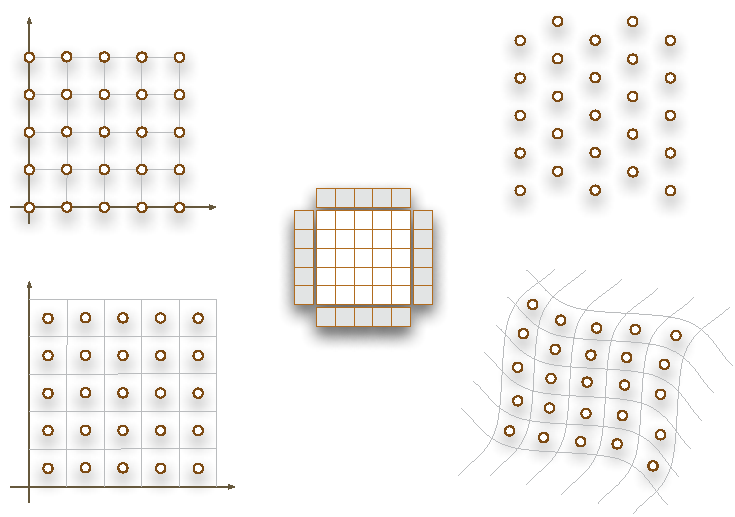
\includegraphics[scale=0.5]{figures/structured.pdf}
  \end{figure} 
%
\end{frame}

% --------------------------------------
% advantages
\begin{frame}[fragile]
%
  \frametitle{Advantages}
%
  \begin{itemize}
%
  \item advantages: logically rectangular
    \begin{itemize}
    \item indexing: easy traversal using loops
    \item fixed stride: predictable memory layout
    \item topology: finding neighbors is trivial
    \end{itemize}
%
    \item disadvantages: many problems don't fit in simple boxes...
      \begin{itemize}
      \item non-trivial geometries are hard to model
      \item the representational simplicity disappears quickly as modeling complexity increases
        \begin{itemize}
        \item domain feature resolution
        \item complex initial and boundary conditions 
        \item adaptive refinement: allowing the properties of the solution to direct where
          computational resources are spent
        \end{itemize}
      \end{itemize}
% 
  \end{itemize}
%
\end{frame}

% --------------------------------------
% data layout
\begin{frame}[fragile]
%
  \frametitle{Data layout and performance}
%
  \begin{itemize}
%
  \item in multi-tier memory architectures
    \begin{itemize}
    \item good data locality enables efficient cache use
    \end{itemize}
%
  \item multi-dimensional arrays: na\"ive implementations do not perform well
    \begin{itemize}
    \item for large problem sizes
    \item for complex physics updates that require keeping track of multiple fields
    \end{itemize}
%
  \item representing scalar, vector and tensor fields
    \begin{itemize}
    \item optimal layout is problem dependent
    \item goal is to minimize cache misses while updating the fields
    \end{itemize}
%
  \item the conventional mapping to arrays lays out the data in matrix form
    \begin{itemize}
    \item not necessarily the most convenient convention
    \end{itemize}
%
  \item take ownership of the indexing function
% 
  \end{itemize}
%
  \begin{figure}
    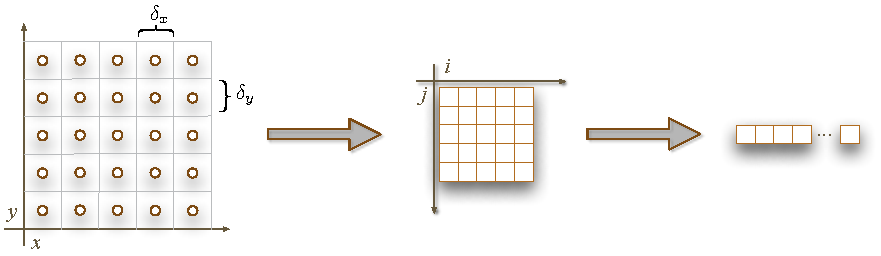
\includegraphics[scale=0.7]{figures/structured-coordinates.pdf}
  \end{figure} 
%
\end{frame}

% --------------------------------------
% updates
\begin{frame}[fragile]
%
  \frametitle{Updating the grid}
%
  \begin{itemize}
%
  \item two broad categories of problems
    \begin{itemize}
      \item steady state problems: iterates represent progress towards enforcing a spatial
        relationship dictated by the differential equation
      \item time dependent problems: iterates represent the time evolution of the solution to
        the spatial problem
    \end{itemize}
%
  \item two broad strategies:
    \begin{itemize}
      \item {\em implicit} solvers cast the constraints among iterates as a large system of
        simultaneous equations
      \item {\em explicit} solvers keep track of only a small number of the iterates
        and use them to advance the solution one step at a time
    \end{itemize}
%
  \item the complexity of the update determines the {\em stencil}
% 
  \end{itemize}
%
  \begin{figure}
    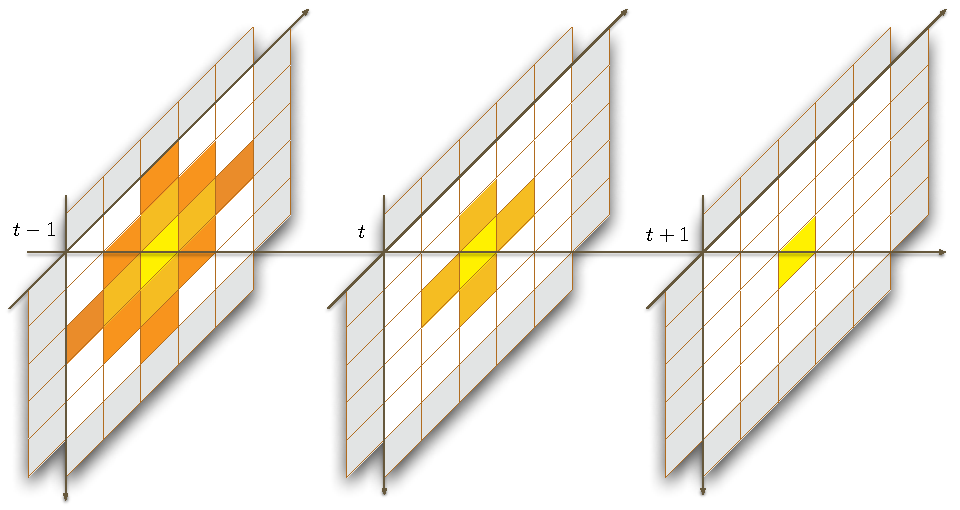
\includegraphics[scale=0.4]{figures/structured-updates.pdf}
  \end{figure} 
%
\end{frame}

% --------------------------------------
% numerics
\begin{frame}[fragile]
%
  \frametitle{Computing derivatives}
%
  \begin{itemize}
%
  \item there are three different first order approximations
    \begin{itemize}
%
    \item forward difference:
      \begin{equation}
      \partial \raisebox{-.4em}{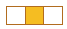
\includegraphics{figures/structured-1d-centered.pdf}}
      =
      \frac{1}{\delta}
      \left(
        \raisebox{-.4em}{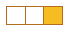
\includegraphics{figures/structured-1d-right.pdf}} 
        -
        \raisebox{-.4em}{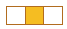
\includegraphics{figures/structured-1d-middle.pdf}} 
      \right)
      \end{equation}
%
    \item backward difference:
      \begin{equation}
      \partial \raisebox{-.4em}{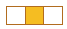
\includegraphics{figures/structured-1d-centered.pdf}}
      =
      \frac{1}{\delta}
      \left(
        \raisebox{-.4em}{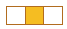
\includegraphics{figures/structured-1d-middle.pdf}} 
        -
        \raisebox{-.4em}{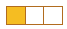
\includegraphics{figures/structured-1d-left.pdf}} 
      \right)
      \end{equation}
%
    \item central difference:
      \begin{equation}
      \partial \raisebox{-.4em}{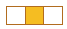
\includegraphics{figures/structured-1d-centered.pdf}}
      =
      \frac{1}{2\delta}
      \left(
        \raisebox{-.4em}{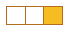
\includegraphics{figures/structured-1d-right.pdf}} 
        -
        \raisebox{-.4em}{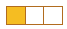
\includegraphics{figures/structured-1d-left.pdf}} 
      \right)
      \end{equation}
%
    \end{itemize}
    where $\delta$ is the uniform grid spacing
%
    \item forward and backward differences are most often used for {\em explicit} time
      integration
%
    \item central differences are used to compute spatial derivatives
%
    \item the second order central difference is given by
      \begin{equation}
      \partial \raisebox{-.2em}{
\includegraphics{figures/structured-1d-5c.pdf}}
      =
      \frac{1}{12\delta}
      \left(
        -
        \raisebox{-.2em}{
\includegraphics{figures/structured-1d-55.pdf}} 
        +
        8 \raisebox{-.2em}{
\includegraphics{figures/structured-1d-54.pdf}} 
        -
        8 \raisebox{-.2em}{
\includegraphics{figures/structured-1d-52.pdf}} 
        +
        \raisebox{-.2em}{
\includegraphics{figures/structured-1d-51.pdf}} 
      \right)
      \end{equation}
%
  \end{itemize}
%
\end{frame}

% --------------------------------------
% numerics
\begin{frame}[fragile]
%
  \frametitle{Partial derivatives in two dimensions}
%
  \begin{itemize}
%
  \item let $\delta_{x}$ and $\delta_{y}$ be the uniform grid spacing along each dimension
%
  \item then, the first order central difference approximations to the spatial derivatives are
    given by
    \begin{eqnarray}
      \partial_{x} \raisebox{-.5em}{
\includegraphics{figures/structured-2d-middle.pdf}}
      & = &
      \frac{1}{2\delta_{x}}
      \left(
        \raisebox{-.5em}{
\includegraphics{figures/structured-2d-e.pdf}} 
        - \raisebox{-.5em}{
\includegraphics{figures/structured-2d-w.pdf}} 
      \right )
      \\
      \partial_{y} \raisebox{-.5em}{
\includegraphics{figures/structured-2d-middle.pdf}}
      & = &
      \frac{1}{2\delta_{y}}
      \left(
        \raisebox{-.5em}{
\includegraphics{figures/structured-2d-s.pdf}} 
        - \raisebox{-.5em}{
\includegraphics{figures/structured-2d-n.pdf}} 
      \right )
    \end{eqnarray}
%
  \item and the second order derivatives are given by
    \begin{eqnarray}
      \partial_{xx} \raisebox{-.5em}{
\includegraphics{figures/structured-2d-middle.pdf}}
      & = &
      \frac{1}{\delta_{x}^{2}}
      \left(
        \raisebox{-.5em}{
\includegraphics{figures/structured-2d-e.pdf}} 
        -2 \raisebox{-.5em}{
\includegraphics{figures/structured-2d-middle.pdf}} 
        + \raisebox{-.5em}{
\includegraphics{figures/structured-2d-w.pdf}} 
      \right )
      \\
      \partial_{yy} \raisebox{-.5em}{
\includegraphics{figures/structured-2d-middle.pdf}}
      & = &
      \frac{1}{\delta_{y}^{2}}
      \left(
        \raisebox{-.5em}{
\includegraphics{figures/structured-2d-s.pdf}} 
        -2 \raisebox{-.5em}{
\includegraphics{figures/structured-2d-middle.pdf}} 
        + \raisebox{-.5em}{
\includegraphics{figures/structured-2d-n.pdf}} 
      \right )
      \\
      \partial_{xy} \raisebox{-.5em}{
\includegraphics{figures/structured-2d-middle.pdf}}
      & = &
      \frac{1}{4\delta_{x}\delta_{y}}
      \left(
        \raisebox{-.5em}{
\includegraphics{figures/structured-2d-se.pdf}} 
        - \raisebox{-.5em}{
\includegraphics{figures/structured-2d-ne.pdf}} 
        - \raisebox{-.5em}{
\includegraphics{figures/structured-2d-sw.pdf}} 
        + \raisebox{-.5em}{
\includegraphics{figures/structured-2d-nw.pdf}} 
      \right )
    \end{eqnarray}
% 
  \end{itemize}
%
\end{frame}

% --------------------------------------
% example
\begin{frame}[fragile]
%
  \frametitle{Solving a simple PDE on a uniform structured grid}
%
  \begin{itemize}
%
  \item Laplace equation over some domain $\Omega \in \mathbb{R}^{d}$, subject to Dirichlet
    boundary conditions
    \begin{equation}
      \begin{array}{ccc}
      \nabla^{2} \phi = 0 & {\rm with} & \phi(\partial \Omega) = f
      \end{array}
      \label{eq:laplace}
    \end{equation}
%
  \item let the grid be uniform: $\delta_{x} =  \delta_{y}$
%
  \item in two dimensions, using first order central differences, \eqref{laplace} becomes
    \begin{eqnarray}
      (\partial_{xx} + \partial_{yy})
      \raisebox{-.5em}{
\includegraphics{figures/structured-2d-middle.pdf}}
      & = &
      0
      \\
      4 \raisebox{-.5em}{
\includegraphics{figures/structured-2d-middle.pdf}} 
      & = &
      \raisebox{-.5em}{
\includegraphics{figures/structured-2d-e.pdf}} 
      + \raisebox{-.5em}{
\includegraphics{figures/structured-2d-w.pdf}} 
      + \raisebox{-.5em}{
\includegraphics{figures/structured-2d-s.pdf}} 
      + \raisebox{-.5em}{
\includegraphics{figures/structured-2d-n.pdf}} 
    \end{eqnarray}
%
  \item and translates into the following constraint among grid elements
    \begin{equation}
      \raisebox{-.5em}{
\includegraphics{figures/structured-2d-middle.pdf}}
      =
      \frac{1}{4}
      \raisebox{-.5em}{
\includegraphics{figures/structured-2d-average.pdf}} 
      \label{eq:laplace-central}
    \end{equation}
    using a shorthand for the sum of the neighboring cells
%
  \end{itemize}
%
\end{frame}

% --------------------------------------
% example
\begin{frame}[fragile]
%
  \frametitle{An example}
%
  \begin{itemize}
%
% 
  \item specifically,
    \begin{itemize}
    \item let $\Omega$ be the unit box in two dimensions
    \item and let $\phi$ satisfy the following boundary conditions
      \begin{equation}
        \begin{array}{rcrcll}
          & & \phi(x,0) & = & \sin(\pi x)           & 0 \leq x \leq 1 \\
          & & \phi(x,1) & = & e^{-\pi} \sin(\pi x)  & 0 \leq x \leq 1 \\
          \phi(0,y) & = & \phi(1, y) & = & 0        & 0 \leq y \leq 1
        \end{array}
      \end{equation}
    \end{itemize}
%
  \item the exact solution is given by
    \begin{equation}
      \phi(x,y) = e^{-\pi y} \sin(\pi x)
    \end{equation}
%
  \item we will solve this equation using the Jacobi iterative scheme:
    \begin{itemize}
    \item make an initial guess for $\phi$ over a discretization of $\Omega$
    \item apply the boundary conditions
    \item interpret \eqref{laplace-central} as an update step to compute the next iteration
      \begin{equation}
      \raisebox{-.5em}{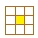
\includegraphics{figures/structured-2d-centered.pdf}}_{t+1}
      =
      \frac{1}{4}
      \raisebox{-.5em}{
\includegraphics{figures/structured-2d-average.pdf}}_{t}
      \end{equation}
    \item stop when a convergence criterion is met
    \end{itemize}
%
  \end{itemize}
%
\end{frame}

% --------------------------------------
% parallelizing
\begin{frame}[fragile]
%
  \frametitle{Implementation strategy}
%
  \begin{itemize}
%
  \item grid resolution:
    \begin{itemize}
     \item ideally determined by analyzing the boundary conditions, since discrete sampling may
       wash out sharp features
     \item for our simple example, this can be done as part of the solver initialization
     \item we will use an $N \times N$ grid and let $N$ be user specified so we can control the
       problem size
       \begin{equation}
         \delta_{x} = \delta_{y} = \frac{1}{N-1}
       \end{equation}
     \end{itemize}
%
  \item data layout
    \begin{itemize}
    \item investigate the effect of data locality by trying out various layouts
    \end{itemize}
%
  \item setting up the update
    \begin{itemize}
      \item we only need to keep track of two iterants
      \item can be done in place; do you see how?
    \end{itemize}
%
  \item convergence criterion
    \begin{itemize}
    \item we will stop iterating when
      \begin{equation}
        \maximum{\Omega} (\phi_{t+1} - \phi_{t})) < \epsilon
      \end{equation}
      and let the user specify $\epsilon$
    \end{itemize}
%
  \end{itemize}
% 
\end{frame}

%
% \begin{figure}
%   \centering
%   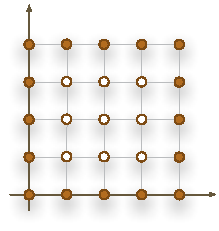
\includegraphics[scale=0.5]{figures/structured-dirichlet.pdf}
% \end{figure}

% --------------------------------------
% parallelization
\begin{frame}[fragile]
%
  \frametitle{Parallelization}
%
  \begin{itemize}
%
  \item the finest grain of work is clearly the cell update based on the value of its four
    nearest neighbors
%
  \item the shared memory implementation requires
    \begin{itemize}
    \item a scheme so that threads can update cells without the need for locks
    \item while maximizing locality of data access
    \item even the computation of the convergence criterion can be parallelized
    \end{itemize}
%
  \item with \mpi
    \begin{itemize}
    \item must partition the mesh among processes
    \item each process work on its own subgrid
    \item communication is required every iteration
    \item parallel convergence testing involves a collective operation
    \end{itemize}
%
  \end{itemize}
%
  \begin{figure}
    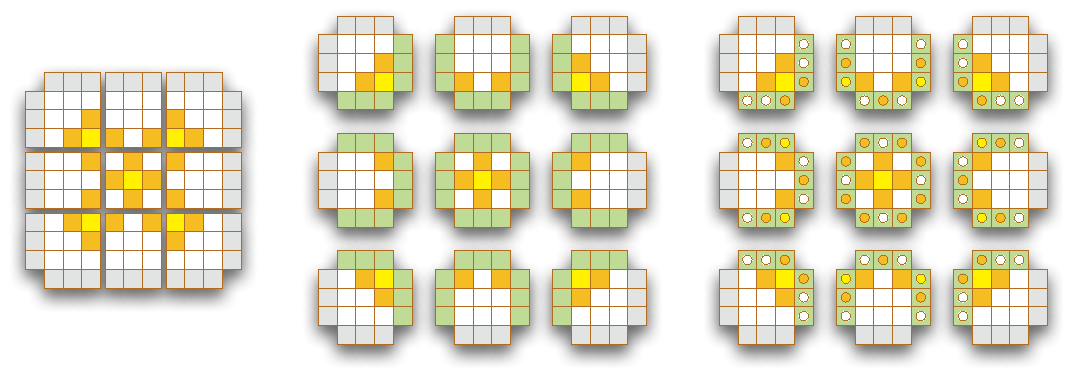
\includegraphics[scale=0.4]{figures/structured-partitioning.pdf}
  \end{figure} 
% 
\end{frame}

% --------------------------------------
% sequential
\begin{frame}[fragile]
%
  \frametitle{Sequential implementation - user interface}
%
  \begin{lstlisting}[language=c++,name=seq:frame,firstnumber=77]
// main program
int main(int argc, char* argv[]) {
    // default values for our user configurable settings
    size_t N = 10;
    double tolerance = 1.0e-6;
    const char* filename = "laplace.csv";

    // read the command line
    int command;
    while ((command = getopt(argc, argv, "N:e:o:")) != -1) {
        switch (command) {
        // get the convergence tolerance
        case 'e':
            tolerance = atof(optarg);
            break;
        // get the grid size
        case 'N':
            N = (size_t) atof(optarg);
            break;
        // get the name of the output file
        case 'o':
            filename = optarg;
        }
    }
    
  \end{lstlisting}
% 
\end{frame}

% --------------------------------------
% sequential
\begin{frame}[fragile]
%
  \frametitle{Sequential implementation - driving the solver}
%
  \begin{lstlisting}[language=c++,name=seq:frame]
    // allocate space for the solution
    Grid potential(N);

    // initialize and apply our boundary conditions
    initialize(potential);

    // call the solver
    laplace(potential, tolerance);

    // open a stream to hold the answer
    std::fstream output(filename, std::ios_base::out);

    // build a visualizer and render the solution in our chosen format
    Visualizer visualizer;
    visualizer.csv(potential, output);

    // all done
    return 0;
}
  \end{lstlisting}
% 
\end{frame}

% end of file 
